\section{Related Work}
\label{sec:related_work}

\paragraph{Training-free LLM IE.}
\looseness=-1
Training-free LLM IE spans instruction tuning \citep{instructuie-2023}, code-style schema encoding \citep{knowcoder-2024,codeie-2023}, annotation-guided extraction \citep{gollie-2024,adelie-2024}, schema-driven decoding \citep{slot-2025,oneke-2025}, and constrained JSON decoding \citep{json-schema-bench-2025,willard2023efficient}. NER methods include zero-shot decomposition \citep{xie-zeroshot-ner-2023,promptner-2023}, distillation \citep{uniner-2024}, and bidirectional encoders \citep{gliner-2024,gliner2-2025}; RE methods include zero-shot triplet extraction \citep{relationprompt-2022}, constrained generation \citep{josifoski-2022-genie}, and shared embedding spaces \citep{boylan-2025-glirel,wadhwa-re-llm-2023}. Related work exploits type embeddings for retrieval \citep{shachar-2025-ner-retriever} and introspective confusion for example selection \citep{reflect-learn-2026}. These methods handle moderate schemas (4--20 types) but none investigates how performance degrades as schema complexity scales.

\begin{figure}[t]
\centering
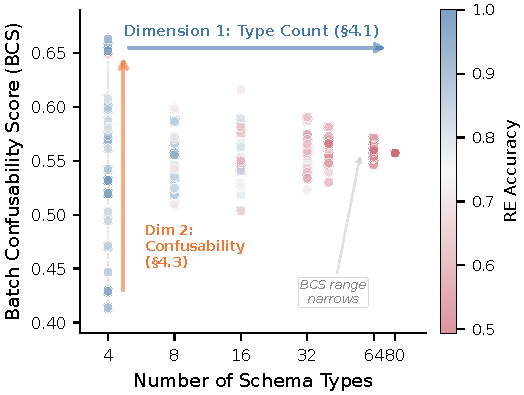
\includegraphics[width=\columnwidth]{../../figures/paper/fig_framework.pdf}
\caption{Experimental design overview on FewRel. Each point is one batch; color encodes RE accuracy (green=high, red=low). \textbf{Dimension~1} (horizontal): accuracy declines with type count (\S\ref{sec:count_curves}). \textbf{Dimension~2} (vertical): within each count level, higher BCS correlates with lower accuracy (\S\ref{sec:bcs_controlled}). BCS range narrows at high counts, limiting Dimension~2 discriminability.}
\label{fig:framework}
\end{figure}

\paragraph{Schema complexity in IE.}
\looseness=-1
The most directly related work is LLM-PEE \citep{llm-pee-2025}, which partitions large event schemas by type embedding similarity. Our work differs in three ways: (1)~we conduct controlled analysis to understand \emph{why} extraction degrades rather than developing an engineering solution; (2)~our BCS-controlled experiments isolate count from confusability with verified orthogonality ($\text{VIF}=1.18$), which LLM-PEE conflates without controlling for confounding variables; (3)~our decomposition experiments (\S\ref{sec:sdgd}) reveal that merge amplification (not partitioning quality) is the bottleneck in decompose-then-merge pipelines. LLM-PEE's union merge suffers the same precision collapse (0.56$\to$0.21; \S\ref{sec:sdgd}). In short, LLM-PEE assumes decomposition helps; we show why it should (confusability), why it does not (merge amplification), and what predicts the degradation (BCS). Other approaches address schema complexity via hard negative mining \citep{iepile-2024}, schema definition optimization \citep{parse-2025}, multi-agent debate \citep{crossagentie-2025,cmas-ner-2025}, and active prompting \citep{reflect-learn-2026}; all treat it as an engineering problem rather than isolating degradation factors. Concurrently, \citet{chen-2026-multi-instance} show that instance count degrades LLM multi-instance processing more than context length, consistent with our count-dominant finding. \citet{golde-2025-familiarity} quantify training--evaluation type similarity to predict zero-shot NER difficulty; our SCS instead measures within-schema inter-type confusability without assuming access to training data. Label-space reduction approaches \citep{haystack-to-needle-2025,dlisc-2025,spt-2025} implicitly lower batch confusability; our framework explains \emph{why} such reduction works.

\paragraph{Schema complexity beyond IE.}
\looseness=-1
Schema-dialogue benchmarks \citep{rastogi2020towards,lee2022sgd} and \citet{li2023evaluating} document count-dependent LLM IE degradation. The link between label similarity and confusion has precedent in vision \citep{dubey-2018-pairwise-confusion,deng-2010-imagenet} and label noise \citep{collier-2021-correlated-noise,guo-2021-label-confusion}.

\paragraph{SCS novelty.}
\looseness=-1
SCS inherits the embedding-similarity criterion from LLM-PEE \citep{llm-pee-2025}, repurposed from schema partitioning to controlled analysis; parallels exist in metric learning \citep{snell2017prototypical} and zero-shot classification \citep{yin-2019-zero-shot-bench}. The modest pairwise $r^2$ (1.3--1.7\%) compounds at the batch level to explain substantial cross-batch RE variance (\S\ref{sec:bcs_controlled}).

\begin{table}[t]
\centering
\small
\resizebox{\columnwidth}{!}{%
\begin{tabular}{llrrlll}
\toprule
\textbf{Dataset} & \textbf{Task} & \textbf{\# Types} & \textbf{\# Eval Units} & \textbf{Domain} & \textbf{BCS Range} & \textbf{Embedding} \\
\midrule
Few-NERD & NER & 66 & 1{,}000 & Cross & 0.77--0.93 & Qwen3-32B \\
FewRel & RE (sent.) & 80 & 1{,}000 & Cross & 0.42--0.97 & MiniLM \\
DocRED & RE (doc.) & 96 & 1{,}000 & Cross & 0.53--0.73 & MiniLM \\
MAVEN & ED & 168 & 18{,}904\rlap{$^\dagger$} & Same & 0.87--0.97 & MiniLM \\
\bottomrule
\end{tabular}}
\caption{Dataset statistics. BCS Range: min--max over count-curve batches. Embedding: model used for SCS/BCS; ranges are not comparable across embedding models. $^\dagger$Trigger mentions across 8{,}042 sentences.}
\label{tab:datasets}
\end{table}

